%%%%%%%%%%%%%%%%%%%%%%%%%%%%%%%%%%%%%%%%%%%%%%%%%%%%%%%%%%%%%%%%%%% 
%                                                                 %
%                            CHAPTER FOUR                         %
%                                                                 %
%%%%%%%%%%%%%%%%%%%%%%%%%%%%%%%%%%%%%%%%%%%%%%%%%%%%%%%%%%%%%%%%%%% 
 
\chapter{NUMERICAL RESULTS: TESTS AND APPLICATIONS}\label{chap:tests}
%\resetfootnote %this command starts footnote numbering with 1 again.
The goal of this chapter is to verify and apply the matrix-free RSNK optimization algorithm described in Chapters~\ref{chap:homotopy} and \ref{chap:linsys}.   We begin by summarizing the software implementation of the proposed algorithm.  We also describe the established algorithm we will compare against.  Next, we use the well-established CUTEr test set to verify the algorithm.  We then present the results of applying the algorithm to two large-scale PDE-constrained optimization problems.


%In our preconditioner, we use a parameter $\mu_e$ 
%   to determine when to switch from approximate to exact second-order adjoints.
%    Only after $\mu \leq \mu_e $ are the exact second-order adjoints are used in the preconditioner 
%   to save computational cost. 

\section{Software Implementation and Benchmarking}

This section begins with an overview of Kona, the software library in which the algorithms from Chapters~\ref{chap:homotopy} and~\ref{chap:linsys} are implemented.  This is followed by a descrption of the convergence criteria used in the matrix-free algorithm. Lastly, we provide a description of SNOPT, an independent and popular optimization library against which we will compare Kona.

\subsection{The Kona Optimization Library}\label{sec:kona_mv}
The globalized RSNK method and preconditioners are part of 
an in-house optimization package, Kona~\cite{dener:scitech2016}. Kona is a matrix-free, 
architecture-agnostic optimization package designed to solve reduced-space PDE-constrained 
optimization problems.  Kona implements several optimization 
algorithms including an unconstrained 
reduced-space quasi-Newton method, an unconstrained reduced-space 
Newton-CG method, an equality constrained reduced-space Newton-Krylov method 
based on FLECS~\cite{hicken:flecs2014}, and an equality-constrained composite-step RSNK algorithm.
These high-level optimization algorithms are built from modular components that implement various optimization subroutines including:
iterative matrix-free solvers like FGMRES, STCG, FLECS for solving linear systems; 
globalization techniques like trust-region, backtracking line search, and a line search based on 
the strong Wolfe conditions;   and merit functions like the augmented Lagrangian and the $l_2$ 
merit function.  In addition, Kona can evaluate Hessian- and Jacobian-vector products by solving the approriate adjoint equations. 

Architecturally, Kona uses an abstract interface to separate the optimization algorithms from PDE-solver specific implementations, and this allows the development of new optimization algorithms independent of the PDE solver. 
 From a user's perspective, one has to write a solver interface to Kona providing 
the function operations listed in Table 4.1 of~\cite{dener_thesis_2017}. In particular, this solver interface 
provides the objective, constraint, gradient, Jacobian-vector, and vector-Jacobian products.
These products allow Kona to evaluate more complex total sensitivities (\eg Hessian- and Jacobian-vector products)
that are needed for RSNK algorithms.


%During the optimization process, 
%conventional gradient-based optimizers rely on sensitivity information to decide how to improve the design from one iteration to the next. In the context of reduced-space PDE-constrained optimization, these sensitivities must be total derivatives that account for the dependence of the state on the design. 


%In contrast, the solver interface 
%required by Kona is designed specifically for PDE-constrained optimization problems by providing 
%partial instead of total gradients for the constraints, matrix-vector products with the system matrix of 
%the PDE solvers, matrix-vector products with the constraint Jacobians w.r.t. the state variables, and the design variables. 
%These matrix-vector products 
%with the Jacobians are used to assemble the matrix-vector products with the Lagrangian Hessian 
%and the total constraint gradients, which in turn are used by the Krylov solvers to solve the linear systems.    

%Although the globalized RSNK's strength is in PDE-constrained optimization area with 
%state variables, it can still be used on problems without the state variables, where the conventional 
%optimization methods dominate.  For such problems, the total gradients are usually cheap to 
%calculate and readily available. For instance, to solve a linear system involving the total constraint Jacobian, 
%conventional optimization methods would ask to compute and 
%store these total gradients for once, then find the solution using direct linear algebra methods. 

%In contrast, the globalized RSNK method would ask to calculate the matrix-vector 
%products with the linear system matrix several times in order to form the Krylov subspace. Each time the constraint Jacobian is 
%calculated and multiplied with an incoming vector. 
%So it's the memory cost of the storage of the matrix versus the computational cost of matrix-vector products 
%for several times. 
%For some problems, the matrix exists in the form of basic algebraic operations, saving the memory cost of storing the matrix even for once. 
\subsection{Convergence Criterion and Default Parameters}
To measure the progress of the optimization iterations, Kona evaluates the infinity
norm of each block row in $F(x)$. Specifically, we will refer to optimality,
complementarity, and feasibility as defined below:
\begin{align*}\label{eq:optfeas}
\text{Optimality} &= \max_{j} | (\nabla_x \mathcal{L})_j |,  \\           % \lVert   \nabla_x f(x) + \lambda^T \nabla_x g(x)  \rVert _{\infty} \\
\text{Complementarity} &= \max_{j} | s_j \lambda_j |,     \\            % \lVert   -\mat{S}\mat{\Lambda} e   \rVert _{\infty}   \\
\text{Feasibility} &=  \max_{j} |   c_j     |  , \quad \text{where} \quad c = \left[ h(x)^T,  (g(x) - s)^T \right].         % \begin{Vmatrix} h(x) g(x) - s  \end{Vmatrix} _{\infty} 
\end{align*}

%$\max_{j} | (\nabla_x \mathcal{L})_j |$

In the subsequent tests, the convergence plots display the above metrics versus
computational cost.  In the past we have reported the relative convergence criteria, which normalizes the above quantities by their initial values; however, in the tests below we report the absolute criteria.
The relative convergence criteria is not appropriate in the current context, because the
 initial complementarity products are zero due to the zero initial multipliers, 
 and the initial feasibility could be zero if $s_0 = g(x_0)$ is used for inequality-only constrained problems. 

Table \ref{tab:param} in Appendix shows the complete list of the parameters used in the test problems, including
the default values set in the algorithm and their recommended ranges.



\subsection{SNOPT}
We will benchmark the performance of Kona against the software library
SNOPT, which is short for Sparse Nonlinear OPTimizer~\cite{gill:2002}. SNOPT is a gradient-based sequential 
quadratic optimization method for solving large-scale nonlinear problems 
with thousands of constraints and design variables. It uses an augmented Lagrangian 
merit function, and the Hessian of the Lagrangian is approximated
using a limited-memory quasi-Newton method. 

SNOPT uses scaled feasibility and optimality criteria 
 to measure the progress of the 
optimization iterations. The feasibility criterion measures the maximum nonlinear constraint violation, 
and is normalized by the norm of the current estimated solution, denoted $x^{(k)}$ below:
\begin{equation*}
\text{SNOPT feasibility} = \underset{i}{\text{max}}  \  c_i / \lVert x^{(k)} \rVert, \quad \text{where} \quad 
c = \left[ h(x)^T,  (g(x) - s)^T \right].  %c= \left[ ( c(x) - cl)^T, (cu -c(x) )^T \right]   
\end{equation*}        
where $x$ is the current iterative point, and 
$c_i$ is the violation of the $i$th nonlinear constraint~\cite{snopt_manual}. SNOPT's feasibility tolerance, 
$\epsilon_r$, has a default value of $10^{-6}$. %defined in Appendix~\ref{sec:cuternm}. 

The optimality criterion measures the maximum complementarity slackness for the design variables, 
and it is calculated using the following formulas:
\begin{equation*}
\text{SNOPT optimality} = \underset{j}{\text{max}}  \ \text{Comp}_j / \lVert \pi \rVert 
\end{equation*}
where  $\pi = [\lambda_h^T, \lambda_g^T]^T$ is the Lagrangian multiplier vector; 
$\text{Comp}_j$ measures the complementarity slackness for the $j$th variable and is defined by:
\begin{equation*}
\text{Comp}_j = \begin{cases}
(\nabla_x \mathcal{L})_j \text{min} (x_j - l_j, 1)  \quad \text{if} \ (\nabla_x \mathcal{L})_j \geq 0 \\
-(\nabla_x \mathcal{L})_j \text{min} (u_j - x_j, 1) \quad \text{if} \ (\nabla_x \mathcal{L})_j < 0
\end{cases}
\end{equation*}
where $l_j$ and $u_j$ denote the lower and upper bounds on the $j$th variable. 
%where $d_j = g_j - \pi^T a_j$ is the gradient of the Lagrangian, $g_j$ is the $j$th objective gradient, 
%$a_j$ is the $j$th constraint Jacobian, $\pi$ is the dual variables. 

\section{CUTEr Test Problems}\label{sec:cuter1}
We have chosen to verify the algorithms presented in Chapters~\ref{chap:homotopy} and~\ref{chap:linsys}  using the CUTEr test problem set ~\cite{cuter_opt, cuter_gould}. This section begins with a brief description of the CUTEr test suite, and then it presents the results of applying Kona and SNOPT to a subset of the CUTEr problems.
The CUTEr problem set, its interface, and its classification methods are discussed in Appendix~\ref{sec:cuternm}, \ref{sec:konacut} and \ref{sec:cuter_clas}.  

\subsection{Problem Description}
The CUTEr set is a collection of 
test problems to test new optimization codes and develop new algorithms. The problem set ranges from small differentiable unconstrained problems to large-scale dense and sparse problems with both equality and inequality nonlinear constraints.
Some of the test problems exhibit challenges and numerical difficulties observable in practice, such as bad scaling in the objective and/or constraint functions, multiple local solutions, non-regular solutions where the linearly-independent constraint qualification is not satisfied, etc. A number of optimization packages have interfaced with CUTEr~\cite{cuter_interface}, including Ipopt, Knitro, Minos, and SNOPT, to name a few.
%  ill-conditioned \textbf{Jacobians}

The problems are written in the so-called Standard Input Format (SIF)~\cite{Conn1992}. A decoder translates the problems written in SIF to a library written in Fortran 77 that provide the tools to access the function values, Jacobians, and, sometimes, Hessians to the optimization packages. %It is important for a developing optimization algorithm to test on a good, quality, and suitable subset of problems in CUTEr/CUTEst to validate its accuracy and robustness. 

\subsection{Results}
As the CUTEr test problem set contains a large collection of problems with assorted features, some of which are inappropriate for the RSNK algorithm, only a subset of the problems are considered here. The following criteria were used to remove certain problems from being considered in the tests; see Appendix~\ref{sec:cuter_clas} for further details on the classification of the CUTEr problems. 
\begin{itemize} \itemsep -8pt 
\item Objective functions with the following type: \textbf{U},  \textbf{C}, and \textbf{L}
\item Constraint functions with the following type: \textbf{U},  \textbf{X}
\item Irregular problems 
% \item Large number of design and constraints, more than a few hundreds
\item Problems with no correct solutions provided
\end{itemize}   %$m_{\text{eq}}$,  $m_{\text{ineq}}$

Table~\ref{tab:cuter} lists the results on the selected subset of the Cuter problems. The first column, `Name' , lists the name of the problems 
as found in the ASCII files from~\cite{cuter_probs}.  The files from~\cite{cuter_probs} also include the
problem origin, authors, classifications, SIF problem cards, and, sometimes, the solutions. The second column `n,  $m_{\text{CUTEr}}$, l, m' are the number of design variables, the number of constraints as described in Appendix~\ref{sec:cuternm}, and the number of equality and inequality constraints as defined in this thesis. 
The third column provides the origin of the problem, if available. The fourth column lists the parameters used in the homotopy RSNK algorithm that were changed for some of the problems: the initial step size $\textbf{$\alpha_0$}$, the nominal distance  $\delta_{\text{targ}}$  and nominal angle $\phi^{\circ}_{\text{targ}}$ as defined in Section~\ref{sec:step}, and the rank of the SVD approximation in Lanczos method used in the preconditioner~\ref{eq:svd}. The fifth column is the optimal value of the  objective function found using Kona, while the sixth column is optimal objective value found using SNOPT. The last column is the optimized objective function value as provided by Reference~\cite{cuter_probs}. 

The results in Table~\ref{tab:cuter} suggest 
that the globalized RSNK algorithm and the preconditioners proposed in this thesis can deliver accurate solutions. They even succeed in a few cases where SNOPT fails. Despite this success, several points are worth highlighting:
\begin{enumerate}\itemsep -2pt
%\item As a majority of CUTEr test problems do not involve state variables, except for a small sets of optimal control problems, the globalized RSNK algorithm loses its edge in saving the computing and storing costs for the constraint Jacobians. Therefore, on average, the globalized RSNK takes longer time than SNOPT to solve the CUTEr problems. 
\item CUTEr is only used as verification here, and it is not intended to demonstrate the efficiency of the RSNK algorithm.  Indeed, the CUTEr test problems are sufficiently small in size and have explicit Jacobians, so these problems do not benefit from the matrix-free RSNK algorithm.

\item The parameters \textbf{$\alpha_0$},  $\delta_{\text{targ}}$, $\phi^{\circ}_{\text{targ}}$,  $n_{\mat{\Sigma}}$ play important roles in the robustness and efficiency of the new algorithm. In some cases the parameters have to be changed manually to get convergence. In contrast, the parameters for SNOPT remained unchanged for all the test problems. 
\item The globalized RSNK algorithm is based on the constraint qualification assumption; therefore, it will fail for problems with redundant constraints.    
\item If the null space of the inequality constraint Jacobian includes a vector of ones, the preconditioner will fail.  Because Kona starts the Lanczos algorithm (used to build the preconditioner) with a vector of ones, 
for problems whose inequality constraint Jacobian contain certain structures, \eg $[-1, -3, 3, 1]$ on each row, the Lanczos method will crash as the matrix vector product is zero. 
 
% For the problems whose inequality constraint Jacobian has a certain structure, \eg $[-1, -3, 3, 1]$ on each row like the LISWET problems, the matrix vector product will be zero, causing the Lanczos method to crash. 
\end{enumerate} 


\begin{landscape}
\begin{longtable}{l | l |  l  |  >{\footnotesize}p{3cm} | l | l | l    }      %\toprule      % |  >{\centering}m{3.5cm}
\caption{Subsets of Cuter Problem Results}\label{tab:cuter} \\
 \hline 
Name      &  n,  $m_{\text{CUTEr}}$, l,  m        &     Origin      &\textbf{$\alpha_0$},  $\delta_{\text{targ}}$, $\phi^{\circ}_{\text{targ}}$,  $n_{\mat{\Sigma}}$      & $ f_{\text{kona}} $   & $ f_{\text{snopt}} $ &$ f^*$    \\ \hline
AIRPORT    &  84,  42, 0, 210  &    &  0.05, 20, 20, 40 & 47952.976  & 47952.702  & 47952.696   \\ \hline
BIGGSC4    &  4, 7, 0, 21  &    & 0.05, 1, 5, 2  &  -24.49999  & -24.375   & -24.5    \\ \hline
BLOCKQP1 &  25, 11, 10, 71  &     & 0.05, 1, 5, 2 & 2.403846   & 2.4038461  &  -6.4988    \\ \hline
BLOCKQP2  &  25, 11, 10, 71  &     & 0.05, 1, 5, 2 & -6.20165    & -2.5e+14  & -6.2017    \\ \hline
%BLOCKQP3 &  25, 11, 10, 71  &     &  0.05, 1, 5, 2  &  2.330508  & 2.330508   & -2.4987e-1     \\ \hline
%BLOCKQP4 &  25, 11, 10, 71  &     &  0.05, 1, 5, 2  &  -2.928928   & -5.7e+14   &  -0.60    \\ \hline
%BLOCKQP5 & 25, 11, 10, 71  &     &  0.05, 1, 5, 2 & 2.330508  &   2.330508   &  -2.4987e-1     \\ \hline
BLOWEYA &  22, 12, 12, 46  &      &   0.05, 1, 5, 10  & -4.56931  & -4.56931   & -4.56932   \\ \hline
% BLOWEYB & 22, 12, 12, 46  &    &  0.05, 1, 5, 10  & -3.05613 &  -3.05613  & -4.93517e2  \\ \hline
% BLOWEYC & 22, 12, 12, 46  &    &  0.05, 1, 5, 10  &-3.06104 & -3.06104 & -2.388E+02 \\ \hline
BT1    &   2, 1, 1, 2  & &  0.05, 10, 20, -    &  -0.99999  & -0.99999   & -1   \\ \hline
BT2    &3, 1, 1, 2  & & 0.05, 10, 20, -   & 0.032568  &  0.032568  & 0.0325682  \\ \hline
BT3    &5, 3, 3, 6 & & 0.05, 10, 20, -   &  4.093013  &  4.093023  & 4.093011 \\ \hline
BT4   &     3, 2, 2, 4 & & 0.05, 10, 20, -   & -45.5106  &  -45.5105  & -45.5105  \\ \hline
BT5   &   3, 2, 2, 4  & non-convex& 0.05, 10, 20, -  & 961.7152  &  961.7152  & 961.7152    \\ \hline
BT6  &  5, 2,2, 4  &  & 0.05, 10, 20, -  & 0.277045  & 0.277045  & 0.277045   \\ \hline
BT7  &  5,3, 3,6   & & 0.05, 1, 10, -   & 306.4957 & 360.3797  & 306.4964  \\ \hline
BT8  & 5,2,2,4   & & 0.05, 1, 10, -  & 1.000000  & 1.000000  & 1   \\ \hline
BT11 &  5,3,3,6  & & 0.05, 1, 10, -  &  0.824892 &  0.824892 & 0.824892   \\ \hline
BT12  &   5,3, 3,6 &&  0.05, 1, 10, - & 6.188113 &  6.188119 & 6.188119   \\ \hline
CHAIN & 102, 51, 51, 106 & &     0.05, 10,20,50 & 5.07047 & -25473973 & 5.07226  \\ \hline
CHANDHEQ &  10, 10, 10, 30 & &  0.05, 10,20,10 & 0  & 0  & 0   \\ \hline
DIPIGRI &7,4,0,4  & & 0.05,10,20, 7  &  680.6301 &  680.6301 & 680.63   \\ \hline
DTOC1L &  58, 36, 36, 80 & DTOC & 0.05,10,20,30 &0.0735945   &0.0307271  & 0.0735931 \\ \hline
DTOC1NA &  58, 36, 36, 80 &non-convex  & 0.05,10,20,30&  0.0753143   &0.0320512  & 0.0753126 \\ \hline
DTOC1NB & 58, 36, 36, 80 &non-convex   & 0.05,10,20,30 &0.0984835   &0.0524561  & 0.0984812 \\ \hline
DTOC1NC & 58, 36, 36, 80 & non-convex  & 0.05,10,20,30 &0.3123065    & 0.2703142   &  0.3123101 \\ \hline
DTOC1ND &  58, 36, 36, 80 & non-convex  & 0.05,10,20,30& 0.4155301   &  0.3845229   &  0.4142563 \\ \hline
DTOC2 &  58, 36, 36, 80 & non-convex  & 0.05,10,20,30 &     0.4859889   &  1.5e-09  &  0.4859839 \\ \hline
DTOC3 &  29, 18, 18, 40 & convex  & 0.05,10,20,30      &     224.59038   &  8.2e-13  &  224.59038 \\ \hline
DTOC4 & 29, 18, 18, 40 &non-convex  & 0.05,10,20,30&      3.7508222  &   1.6e-13  &  3.7507839 \\ \hline
DTOC5  &  19, 9, 9, 20 &convex  & 0.05,10,20,30 &  1.451900  &   4.4e-13  & 1.4518939 \\ \hline
DTOC6 &  19, 9, 9, 20 &convex  &  0.05,10,20,30 & 19.80411 &  9.740196 & 19.80411 \\ \hline
% DUAL1 &  85, 1,1, 170 &   pc linalg error &  0.05,10,20,2 & 0.0633427 & 0.0339766 &    3.5E-02 \\ \hline
DUAL2 & 96, 1, 1, 192 &    &  0.05,10,20,2 &  3.37546E-2 & 3.36831E-2 &    3.37337E-2 \\ \hline
DUAL3 &  111, 1, 1, 222 &  & 0.05,10,20,1 &1.35542E-1  &    1.35544E-1  &   1.35756E-1\\ \hline
EQC &9, 3, 0, 21 & Quality Control & 0.05,10,20,5 & -4789.377 & -4789.377 & 1138.416 \\ \hline
GILBERT & 2,1,1,1 &  & 0.05,1,10,2  & 0.251624        &  0.251624     &  0.251626 \\ \hline
GILBERT & 5,1,1,1 &  & 0.05,1,10,2  & 1.339713        &  1.339713    &  1.339710 \\ \hline
GILBERT &10,1,1,1 &  & 0.05,1,10,2  & 3.345201       &  3.345201    &  3.345196 \\ \hline
GMNCASE1 &   175, 300, 0, 300  &   optimized control   & 0.5, 5, 5, 100   &   0.267087  & 0.266973             &    0.266733   \\ \hline
GMNCASE4 & 175, 350, 0, 350  &  optimized control &  0.05, 10, 20, 170      & 5.9132e3 &  5.9469e3 &   5.9468e3 \\ \hline 
HS100  & 7, 4, 0, 4 & &0.05,10,20,- &  680.6300 & 680.6300 & 680.6300  \\ \hline
HS100LNP & 7, 2, 2, 0 & & 0.05,10,20,-  &  680.6300 & 680.6300 & 680.6300 \\ \hline
HS104 &   8,5, 0,22 & &  0.05,10,20,3 & 3.951162  &     3.951163 &  3.951163    \\ \hline
HS11  &  2,1,0,1 & & 0.05,10,20,1     & -8.498464 &     -8.498465 & -8.49846   \\ \hline
HS112 & 10,3,3,10 & & 0.05,1,5,3 & -47.7611 &  -47.7611 & -47.7075   \\ \hline
HS113 &10, 8,0, 8 & & 0.05,10,20,1 & 24.30621 & 24.30621 & 24.30621   \\ \hline
HS118 &  15, 17,0, 59 & &  0.05,10,20,- & 664.7021 & -1748.637  & 664.8204  \\ \hline
HS12 &  2, 1,0, 1 & &   0.05,10,20,5 & -30 & -30 & -30   \\ \hline
HS14 & 2,2,1,3 & &   0.05,10,20,1  &   1.393465 &  1.393461               & 1.423224\\ \hline
HS15 &  2,2,0,3 & &   0.05,10,20,1 &    306.5000 & 6.8e-17 & 306.5 \\ \hline
HS16 &  2,2,0,5 & &   0.05,10,20,1    & 0.25 & 3.98 &    0.25 \\ \hline
HS21    & 2,1,0,5   & Schittkowski  &  0.5,5,10,1   & -99.3434  & -99.9900  & -99.96    \\ \hline 
HS35   &   3,1,0,4  &             &  0.05,1,5,1    & 0.111111  & 0.111111   &   0.111111   \\ \hline 
HS35I   &   3,1, 0,7  &             &   0.05,1,5,1      & 0.111111  & 0.111111   &   0.111111   \\ \hline 
HS44   & 4,6, 0,10   &  	 & 0.05,1,20,3      &  -13.000 & -4.01e+14 & -13.0    \\ \hline
HS44NEW & 4,6,0,10  &     &   0.05,1,20,3    & -13     & -3.20e+14   & -13.0    \\ \hline
HS51    &  5,3,3,6    &  & 0.05,1,20,3      & 4.46e-19   & 5.86E-14     & 0.0    \\ \hline
HS52    &  5,3,3,6   & & 0.05,1,20,3      & 5.326634   & 5.326647   & 5.326643   \\ \hline
HS53    &  5,3,3,16    &   &  0.05,1,5,3  & 4.093023   & 4.093023   & 4.093023  \\ \hline
HS118  & 15,17,0,59  & & 0.05,50,5,3   & 664.8205  & -1748.638  &664.8204    \\ \hline
HATFLDH  & 4, 7,0, 21  & & 0.05,1,5,2  &  -24.5002  & -24.375 & 24.5   \\ \hline

MOSARQP1 & 36, 10, 0, 46 &convex quadratic & 0.05,1,5,4 &  -24.1436 & -52.0492 & -24.1377 \\ \hline
MOSARQP2 &36,10, 0, 46 &  &0.05,1,5,4  & -35.6982  &-55.1623  & -35.6981 \\ \hline
STCQP1  & 17, 8, 8, 50 & convex quadratic  & 0.05,1,5,5& 494.4054  & 494.5208  & 494.5209 \\\hline
SOSQP1 &  20, 11, 11, 62 & non-convex  &  0.05,1,5,2 &5.9e-07 & -4E-16   & 0.0 \\\hline
SOSQP2 &  20, 11, 11, 62 &  &0.05,1,5,5	&  -3.99779  & -4.045649  & -3.99781    \\\hline
YAO   &  22, 20, 0, 25 & & 0.05,1,5,10& 2.398829  & 0.0037148 & 2.39883  \\\hline
\end{longtable}   % \midrule
\end{landscape}

%AIRPORT & 84, 42  & 84, 0, 210 & SQR2-MN-84-42  & 0.05,20,20,40 & 47952.97672  & 47953.7026  &    \\ \hline 
%AUG2D    &           24,  9         &  24,   9,  18       &    2-D Laplace   & 0.05,1,5,30   &  0.124999           &     0.1250    &      N/A                \\ \hline
%AUG2D    &          220, 100   & 220, 100, 200  &                      &   0.05,1,5,30         &   110.7987          &    110.7991      &    N/A           \\ \hline
%AUG2DC  &       24, 9      &   24, 9, 18       &       &     0.05,1,5,30        &    2.973213        & 2.973214    &   N/A     \\ \hline
%AUG2DC  &      220, 100   &  220, 100, 200   &     &   0.05,1,5,30    & 184.2388    &   184.2394     &    N/A      \\ \hline
%AUG3D  &      156, 27    & 156, 27, 54   & 3-D Laplace  &  0.05,1,5,30   & 0.08333   &   0.083333   &  N/A         \\ \hline
%AUG3DC  &  156, 27  &  156, 27, 54   &    & 0.05,1,5,30 &   35.84226   &   35.84276      & N/A      \\ \hline
% AVGASA  &       8, 10   &   8, 0, 26   &   \cellcolor{blue}         LP, Integer Variable    &   0.05,1,5,30       &           -4.63092    &    -4.79278   &   N/A     \\ \hline
% AVGASB  &    8, 10  &   8, 0, 26   &   \cellcolor{blue}    LP, Integer Variable   & 0.05,1,5,30   &   -4.482206   &   -4.666351     &   N/A    \\ \hline
%ALLINQP  & 10, 5   &  10, 1, 21   & banded QP  &  0.05,10,20,30 & \cellcolor{blue}0.346667  & \cellcolor{blue}-0.183256     &  N/A \\  \hline     %\midrule
%BLOCKQP2   & 25, 11   & 25,  10, 71   &    non-convex quadratic & 0.05,1,5,5  & -6.201652   &  \cellcolor{yellow}  -2.507e+14    &  \cellcolor{yellow}  -6.2017   \\ \hline
%BLOCKQP3   & 25, 11   & 25,  10, 71  & non-convex quadratic  	  & 0.05,1,5,2 & \cellcolor{blue} 2.330508     &  \cellcolor{blue}2.330508   &            \cellcolor{blue}-2.4987e-1   \\ \hline
%BLOCKQP4  & 25, 11    & 25, 10, 71  &    & 0.05,1,5,5     &\cellcolor{blue} -2.928928   & \cellcolor{blue}-5.73e+14   &    \cellcolor{blue} -0.6   \\ \hline
%BDRY2   & 25, 18   & 25, 18, 86   &  AMPL  & 0.05,1,5,3  & 0.547854  & 0.548110  & N/A    \\ \hline   
%BIGGSC4  & 4, 7   & 4, 0, 21   & & 0.05,1,5,2  & -24.4999   &  -24.375  &    -24.5 \\ \hline 
%CVXQP1  & 10, 5 & 10, 5, 30  & convex   & 0.05,1,5,2 & \cellcolor{blue}181.0401 & \cellcolor{blue}165.8738  & N/A   \\ \hline
%DEGENQP & 10, 1005 & 10,5,2030  & degenerate  $N^3$ cons & 0.05,1,5,10  & 8.80e-06 & -5.55e-17  & N/A \\ \hline
%DTOC3   & 29, 18  & 29,18,40 & discrete time control & 0.05,1,5,10  &  224.5904 & \cellcolor{yellow}8.2e-13  &\cellcolor{yellow} 224.5904 \\ \hline 
%GENHS28 & 10, 8  & 10, 8, 16  & Hock and Schittkowski &   0.05,1,5,2   & 0.927173  & 0.927174  & 0.0   \\ \hline
%GMNCASE1 &  175, 300   & 175, 0, 300  &   optimized control   & 0.5, 5, 5, 100   &   0.267087  & 0.266973             &    0.266733   \\ \hline
%GMNCASE4 & 175, 350 & 175, 0, 350  &  optimized control &  0.05, 10, 20, 170      & 5.9132e3 &  5.9469e3 &   5.9468e3 \\ \hline 
%HS268   & 5,5  & 5, 0, 5  &  Schittkowski   &  0.05,50,5,3    & 2.09e-4   & -3.6e-12      &    N/A    \\ \hline 
%HS21    &  2,1 & 2,0,5   & Hock and  Schittkowski  &  0.5,5,10,1   & -99.3434  & -99.9900  & -99.96    \\ \hline 
%HS35   &  3,1  & 3,0,4  &             &  0.05,1,5,1    & 0.111111  & 0.111111   &   0.111111   \\ \hline 
%HS35I   &  3,1  & 3,0,7  &             &   0.05,1,5,1      & 0.111111  & 0.111111   &   0.111111   \\ \hline 
%HS44   & 4,6   & 4,0,10   &  	 & 0.05,1,20,3      &  -13.000 &\cellcolor{yellow} -4.01e+14 & \cellcolor{yellow}-13.0    \\ \hline
%HS44NEW & 4,6  & 4,0,10  &     &   0.05,1,20,3    & -13     &\cellcolor{yellow} -3.20e+14   &\cellcolor{yellow} -13.0    \\ \hline
%HS51    &  5,3   & 5,3,6    &  & 0.05,1,20,3      & 4.46e-19   & 5.86E-14     & 0.0    \\ \hline
%HS52    &  5,3  & 5,3,6   & & 0.05,1,20,3      & 5.326634   & 5.326647   & 5.326643   \\ \hline
%HS53    &  5,3  & 5,3,16    &   &  0.05,1,5,3  & 4.093023   & 4.093023   & 4.093023  \\ \hline
%HS118  & 15,17  & 15,0,59  & & 0.05,50,5,3   & 664.8205  &\cellcolor{yellow} -1748.638  & \cellcolor{yellow}664.8204    \\ \hline
%HS268  & 5,5  & 5,0,5  & & 0.05,50,5,3     & \cellcolor{blue} 3.839e-4 & \cellcolor{blue}-3E-12  & N/A   \\ \hline
%HATFLDH  & 4, 7 &  4, 0, 21  & & 0.05,1,5,2  &  -24.5002  & -24.375 & 24.5   \\ \hline
%LOTSCHD  & 12,7  &  12, 7, 26 & eco. lot scheduling &  0.05,10,20,10   &  \cellcolor{blue}2398.416 &  \cellcolor{blue}165.6553  & N/A  \\ \hline
%MOSARQP1 & 36, 10 & 36, 0, 46 &convex quadratic & 0.05,1,5,4     &  -24.13771 &  \cellcolor{yellow}-52.04917 & \cellcolor{yellow} -24.13768 \\ \hline
% MOSARQP2 &36, 10 & 36, 0, 46 &     & 0.05,1,5,4   & -35.69815  & \cellcolor{yellow}-55.16234  & \cellcolor{yellow}-35.6981 \\ \hline
%POWELL20 & 10,10  & 10,0,10 & degenerate convex & 0.05,1,5,2    & 57.8125 & 57.8125  & N/A  \\\hline
%RDW2D52F & 18,1  & 18,1,36 & optimal control &  0.05,10,20,5 &  \cellcolor{blue}0.053016 & \cellcolor{blue} 0.020779 & N/A \\\hline
%STCQP1  & 17, 8  &  17, 8, 50 & convex   &    0.05,1,5,5  & 494.4054  & 494.5208  & 4.95E+02 \\\hline
%SOSQP1 &  20, 11 & 20, 11, 62 & non-convex & 0.05,1,5,2    & 5.9e-07 & -4E-16   & 0.0 \\\hline
%SOSQP2 & 20,11  &  20, 11, 62 &    & 0.05,1,5,5	& -3.99779  & -4.04565  & -3.99781    \\\hline
% S268   &   5,5   & 5,0,5  &Schittkowski   & 0.05,10,20,10  &    \cellcolor{blue}2.274e-3  &  \cellcolor{blue} -3.64E-12  & N/A  \\\hline
%YAO   &  22,20  & 22, 0, 25 &   &  0.05,1,5,10 & 2.398829  & \cellcolor{yellow}3.715e-3 & \cellcolor{yellow}2.39883  \\\hline
%ZECEVIC2 & 2,2 & 2,0,6  & &  0.05,1,5,2 & -4.1249  & -4.125  & N/A  \\\hline




\newpage

\section{Stress-Constrained Mass Minimization}\label{sec:fstopo2}
\subsection{Problem Description}
Our next numerical experiment is a PDE-constrained structural sizing problem
with state-based constraints.  The problem was previously considered by the
authors in \cite{dener:scitech2016}, and the geometry and boundary conditions
are illustrated in Figure~\ref{fig:struct}.  Informally, the problem consists of
minimizing the plate mass with respect to the thickness distribution, subject
to bound constraints and the von Mises stress criteria. 
\begin{figure}[H]
  \centering
  \includegraphics[width=0.6\textwidth]{./figs/chap6_fstopo/struct.png}
  \caption{Plate thickness design problem}
  \label{fig:struct}
\end{figure}

The response of the plate to the applied force is modeled using the equations of
linear elasticity assuming 2D plane stress.  The governing equations are
discretized using the finite element method with bilinear elements.
A uniform mesh of $n_x \times n_y$ elements is employed, and the thickness
distribution is piecewise constant over each element.  These thickness values
are taken to be the design variables, so there are $n = n_x n_y$ design
variables.

The formal optimization statement is
\begin{equation*}
  \begin{alignedat}{2}
    \underset{x}{\text{min}} \quad &\textsf{mass}(x) \\  % = \sum_{i=1}^{n} m_i x_i, & &\\
    \text{subject to} \quad &\textsf{stress}_i(x) \leq \sigma_{\max}, &
    &\forall\; i = 1,2,\ldots,n, \\
      & x_l \leq x_i \leq  x_u, \qquad & &\forall\; i = 1,2,\ldots,n,
  \end{alignedat}
\end{equation*}
where $\textsf{mass}(x)$ is the plate mass, and $\textsf{stress}_{i}(x)$ is the
von Mises stress criterion on the $i$th element. The thickness of each element
is bounded by the lower and upper values, $x_l = 0.02$ and $x_u = 0.98$. 

The objective function, $\textsf{mass}(x)$, is a sum of all the elements' mass. 
Each element's mass is obtained by a constant material density times the filtered thickness of that element. 
The filtered thickness of each element is a weighted sum of the design variables 
of the adjacent elements within a conic filter, with the weights determined by 
$1-\frac{r}{r_0}$ and normalized so that the sum is $1$;   the radius of the conic $r_0=2$, and $r$ is the distance 
of the adjacent element to the central element.  In summary, the mass is a linear function
of the design variables and is given by
\begin{equation*}
  \textsf{mass}(x) = \sum_{i=1}^{n} m_{i} \sum_{j} w_{ij} x_j,     % \sum_{i=1}^{n} m_i x_i,
\end{equation*}
where $m_i$ is the mass per unit thickness of the $i$th element of the
structure, and $w_{ij}$ is the weight from the filter. 


The von Mises stress
criterion on the $i$th element can be expressed as
\begin{equation*}
  \textsf{stress}_i(x) = 1 - u(x)^T \mat{B}^T \mat{G} \mat{B} u(x),
\end{equation*}
where $\mat{B} u(x)$ gives the strain as a function of the displacement,
$u(x)$, and $\mat{G}$ is a positive-definite matrix.  The displacement is a
function of the design variables through the discretized governing equation
\begin{equation*}
  R(x,u) = \mat{K}(x) u - b,
\end{equation*}
where $\mat{K}(x)$ is the stiffness matrix and $b$ is the force vector.

We consider a set of three mesh sizes by varying $n_x$ and $n_y$.  Table
\ref{tab:mesh_sizes} lists the mesh dimensions and number of design variables
for the three cases. We will informally refer to these three cases as the small, medium, and large
cases.

\begin{table}[tbp]
  \begin{center}
    \caption{Mesh dimensions ($n_x$ and $n_y$), number of design variables ($n =
      n_x n_y$), and size of the approximate SVD preconditioner
      ($n_{\mat{\Sigma}}$) for the plate-thickness optimization
      problem \label{tab:mesh_sizes}}
  \begin{tabular}{ l c c c c}
    \textbf{Case} & $\mathbf{n_x}$  & $\mathbf{n_y}$ & $\mathbf{n}$
    & $\mathbf{{n_{\mat{\Sigma}}}}$
    \\ \hline
    \rule{0ex}{3ex}%
    Small  &   16 & 8  & 128  & 20 \\ 
    Medium &   32 & 16 & 512  & 80 \\  
    Large  &   64 & 32 & 2048 & 320  
  \end{tabular}
  \end{center}
\end{table}

Table~\ref{tab:mesh_sizes} also lists the number of approximate singular values
used in Algorithm~\ref{alg:precond} to construct the preconditioner.  As the number of design variables
increases in this structural optimization problem, the number of singular values
in the SVD approximation has to increase accordingly, at about $\frac{1}{6}$
of the number of design variables.
%Figure~\ref{fig:svdrank} shows the convergence history of the Krylov iterative
%method applied to \eqref{eq:linsys}.  

\subsection{Effectiveness of Preconditioner}
To show the effectiveness of the proposed preconditioner, 
Figure~\ref{fig:svdrank} plots the convergence history of the Krylov
method when the Lanczos-based preconditioner uses an 
increasing number of SVD ranks. The KKT system is extracted from 
the first Newton step of the final corrector phase 
at $\mu < \epsilon_{\mu}$ (\ie the last homotopy iteration) for the small case. 
The KKT system is most ill-conditioned at the final corrector step, so this particular system provides the most stringent test for the preconditioner.

\begin{figure}[tbp]
  \centering
  \includegraphics[width=1.0\textwidth]{./figs/chap6_fstopo/tiny_svd_ranks.eps}
  \caption{Impact of $\nsig$, the rank of the approximate SVD in
    Algorithm~\ref{alg:precond}, on the Krylov iterative method.
  \label{fig:svdrank}}
\end{figure}

\subsection{Optimal Thickness and Comparison with SNOPT}
The structural optimization problem was solved using the proposed algorithm,
with and without the preconditioner. Convergence histories are compared with 
those of SNOPT in Figures \ref{fig:small}, \ref{fig:med}, and \ref{fig:large} for the 
small, medium, and larges cases, respectively. The cost on the horiztonal axis 
measures the equivalent number of PDE solves, 
\ie, the total CPU time divided by the time needed for one
forward solution.  The vertical axis measures the change in absolute optimality, 
absolute feasiblity, and absolute complementarity.    

\begin{figure}[tbp]
  \centering
   \subfloat[Globalized RSNK with Preconditioner \label{fig:thick}]{
   \includegraphics[clip,width=0.85\textwidth]{./figs/chap6_fstopo/medium_thickness_pc.pdf} }
  \hspace{1em}
  \subfloat[Globalized RSNK without Preconditioner \label{fig:thick_eye}]{
   \includegraphics[clip,width=0.85\textwidth]{./figs/chap6_fstopo/medium_thickness_eye.pdf} }
  \hspace{1em}
    \subfloat[SNOPT \label{fig:thick_snopt}]{
   \includegraphics[clip,width=0.85\textwidth]{./figs/chap6_fstopo/medium_thickness_snopt.pdf} }
    \caption{Optimal thickness distribution using Algorithm~\ref{alg:pc} with Preconditioner, without Preconditioner, and SNOPT \label{fig:thick3}}
\end{figure}



    
The final optimal thickness distribution on the large mesh obtained using the homotopy-globalized RSNK method with SVD preconditioner is plotted in Figure~\ref{fig:thick}; the distribution obtained without the preconditioner is shown in Figure~\ref{fig:thick_eye}; finally, the thickness distribution obtained using SNOPT is shown in Figure~\ref{fig:thick_snopt}. 
The thickness distribution pattern in all three plots is qualitatively similar and in agreement with physical
intuition for this problem. 

However, the solution using the globalized RSNK method with the preconditioner has a sharper resolution than that without the preconditioner. In addition, The thickness distribution using SNOPT is ruffled along the trapezoid edges; this is consistent with the convergence plots of SNOPT in \ref{fig:large} below, which shows that SNOPT is having difficulty converging the large problem. 

%*[clip,trim=20 70 0 70, width=1.0\textwidth]

The convergence histories in Figure~\ref{fig:struct2} highlight the need for preconditioning
on this particular problem: without the approximate-SVD preconditioner, the optimality, complementarity and 
feasibility cannot be sufficiently reduced, despite the fact that the thickness distribution 
still looks reasonable. 
In contrast, when the approximate-SVD preconditioner is used the
proposed algorithm can successfully reduce the optimality 
and feasibility to the desired tolerance.

Figures \ref{fig:small}--\ref{fig:large} also show that the performance of SNOPT
degrades as the problem size increases; on the small problem, optimality is
reduced by only three orders of magnitude, while on the large problem the optimality
fluctuates and struggles to decrease significantly. The feasibility achieved by SNOPT is somewhat better
than its optimality, but it also degrades with problem size.  The proposed
predictor-corrector algorithm is able to converge the optimality and feasiblity
five orders of magnitude on all three problems. We see that the
optimization cost increases approximately linearly with $n$ on this
problem, and the cost is driven primarily by the increasing number of singular values used
in the preconditioner. 

\begin{figure}[tbp]
  \centering
   \subfloat[small \label{fig:small}]{
   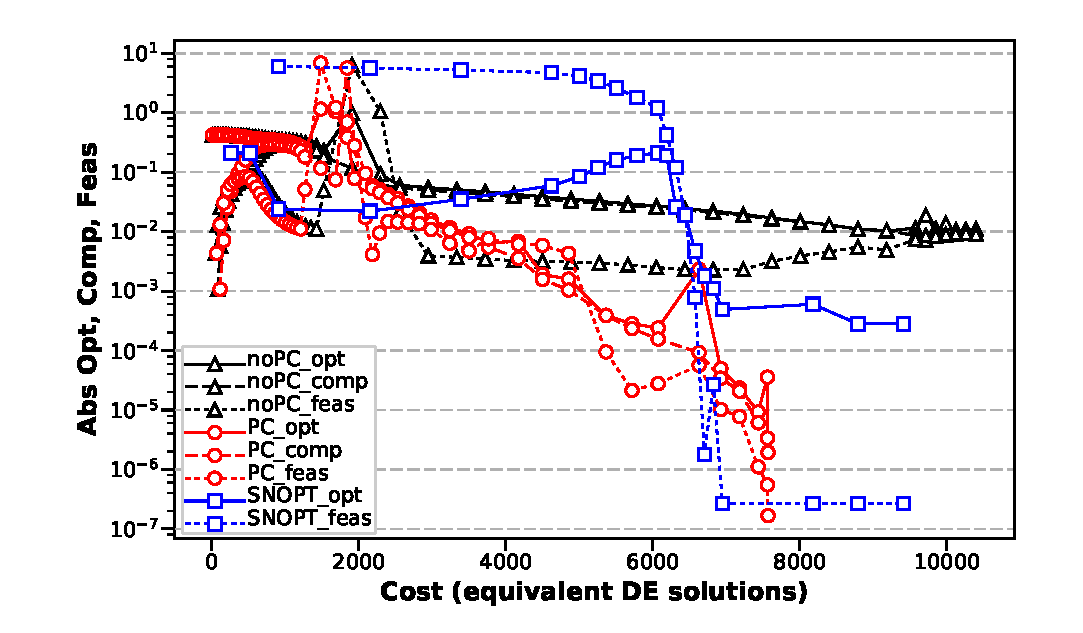
\includegraphics[clip,width=0.8\textwidth]{./figs/chap6_fstopo/tiny_color.eps} }
  \hspace{1em}
  \subfloat[medium \label{fig:med}]{
   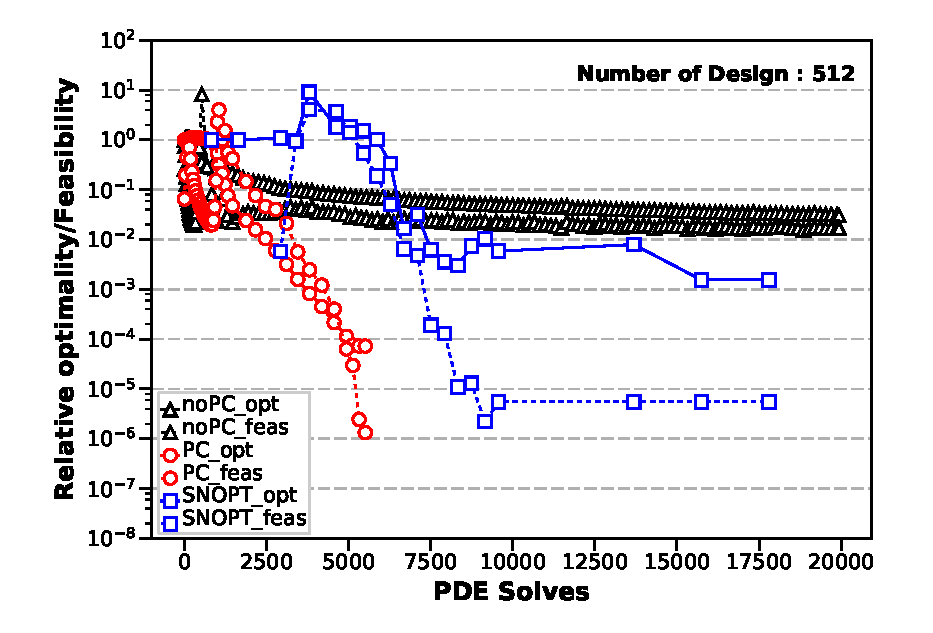
\includegraphics[clip,width=0.8\textwidth]{./figs/chap6_fstopo/small_color.eps} }
  \hspace{1em}
    \subfloat[large \label{fig:large}]{
   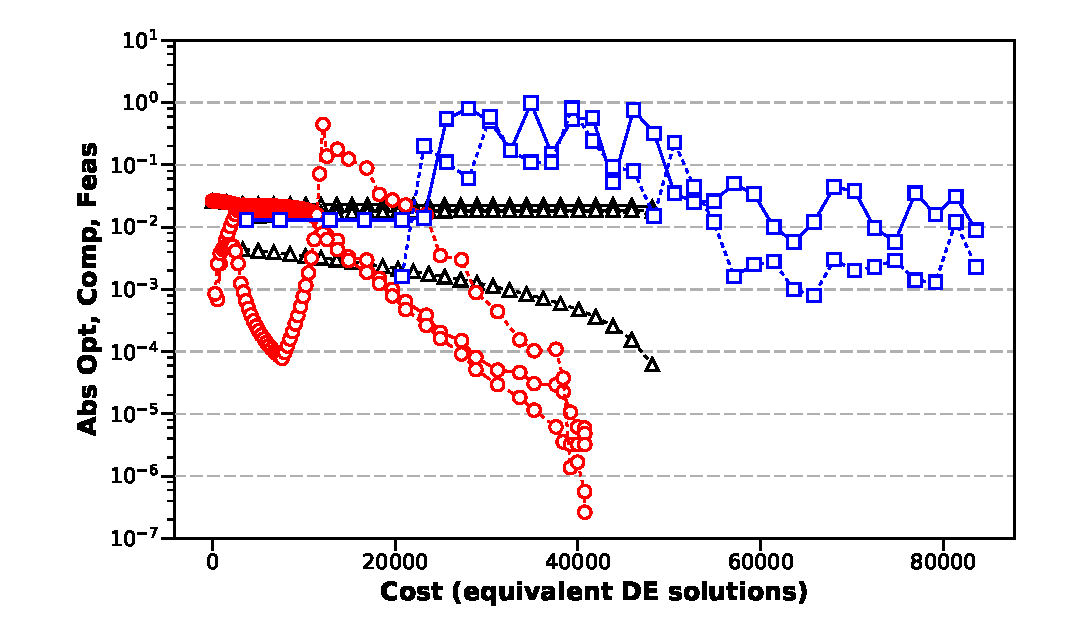
\includegraphics[clip,width=0.8\textwidth]{./figs/chap6_fstopo/medium_color.eps} }
    \caption{Convergence histories for the three sizes of the structural
      optimization problem. \label{fig:struct2}}
\end{figure}

%%%%%%%%%%%%%%%%%%%%%%%%%%%%%%%%%
\newpage
\section{Aerodynamic Shape Optimization}

The last application is an Euler-based aerodynamic shape optimization problem starting from the NASA Common Research Model (CRM) wing~\cite{crm_wing}. This problem is an invisicid version of a problem defined by
the AIAA Aerodynamic Design Optimization Discussion Group (ADODG) ~\cite{adodg}, and involves drag minimization subject to lift, pitching moment, and geometric constraints.   

\subsection{Problem Description}
The baseline wing-only geometry is extracted from the CRM wing-body configuration with a blunt trailing edge. An IGES file is provided to the public as shown in Figure~\ref{fig:crm_wing}. The CRM is modeled after a contemporary transonic commercial airliner, with a size similar to that of Boeing 777. It has been designed with good aerodynamic performance, but with an aggressive pressure recovery on the outboard wing, which provides room for performance improvements. 
%For flight conditions, we use 
%the nominal cruise flight condition for a Boeing 777 which is at Mach 0.85 and a Reynolds number of 5 million based on the mean aerodynamic chord. 

For completeness and repeatability, we provide the following geometric information. 
The origin of the coordinate system is at the leading edge of the wing root, and all coordinates are scaled by the mean aerodynamic chord of 275.8 inches. Pitching moments are measured about the point $(1.2077, 0, 0.007669)$ using the reference length. All aerodynamic coefficients are computed based on the projected area $S_{\text{ref}}=3.407014$ squared reference units. 

\begin{figure}[tbp]
  \centering
  \includegraphics[clip,width=0.75\textwidth]{./figs/chap7_aso/CRM-wing.png}%
  \caption{CRM wing \label{fig:crm_wing}}
\end{figure}


\subsection{Mesh Generation, Parameterization and Flow Solver}
The mesh CGNS file is generated by the University of Michigan's MDOLab's in-house hyperbolic mesh generator, and uses an O-grid topology method from the wing surface to a farfield a distance 25 times the wing span away from the origin. Three levels of mesh are available for Euler cases as shown in Table~\ref{tab:euler_mesh}. 
The results in the table show that the drag coefficient appears to be grid converged on the L1 grid. Therefore, only the L1 grid is used in this study. 

\begin{table}[H]
  \begin{center}
    \caption{Three grid levels and baseline aerodynamic coefficients
    \label{tab:euler_mesh}}
  \begin{tabular}{ c r c c c c }
 \textbf{Mesh level}   &  \textbf{Mesh size}  & $\mathbf{C_D}$ & $\mathbf{C_L} $ & $\mathbf{C_M}$ & $\mathbf{\alpha}$  \\\hline
 L0                  &  840,192   & 0.00995   & 0.49879 & -0.20182  & $2.5^{\circ}$   \\
 L1                  &  105,024   & 0.01085   & 0.48925 & -0.19502    & $2.5^{\circ}$ \\
 L2 		      &   13,000    &  0.01417   & 0.46638    & -0.18142  &  	$2.5^{\circ}$ 	 
  \end{tabular}
  \end{center}
\end{table}

The wing geometry is parameterized using a free-form deformation (FFD) volume method~\cite{Kenway:2010:C}. In FFD, the wing geometry is embedded inside a B-spline volume, and the geometric changes of the wing surface are performed by changing the B-spline control points.
Figure~\ref{fig:crm_ffd} shows the FFD volume and the control points. For the following study, the displacement of the control points in the vertical $z$ direction are used as the design variables. 

 \begin{figure}[tbp]
  \centering
  \includegraphics[clip,width=0.8\textwidth]{./figs/chap7_aso/CRM-wing-FFD.png}%
  \caption{CRM FFD \label{fig:crm_ffd}}
\end{figure}

The flow solver used in this study is SUmb~\cite{sumb_pdf}, a finite-volume, cell-centered multi-block structured  flow solver that can model a variety  of problems, including the compressible Euler, laminar Navier-Stokes and Reynolds-Averaged Navier-Stokes (RANS) equations. In this study, the flow was modeled with the compressible Euler equations. The DRP cluster on Rensselaer Polytechnic Institute's CCI was used, consisting of 64 nodes; each node has 128GB of system memory and two eight-core 2.6 GHz Intel Xeon E5-2650 processors. 

\subsection{Optimization Problem Statement}
During the optimization, the wing's sectional shape and twist are altered 
by changing the vertical $z$ coordinates 
of the FFD control points. The control points are distributed in $n_x$ chord wise locations and across  $n_y$ spanwise sections;  see Figure~\ref{fig:crm_ffd}. The leading and trailing edges of the root section are fixed. For the other sections, the trailing edge is fixed while the leading edge is free. This permits arbitrary wing twists to be implicitly represented by the remaining degrees of freedom. The wing planform is fixed because the $x$ and $y$ coordinates of the FFD control points are fixed. The angle of attack is one of the design variables and is permitted to change.  

The optimization problem can be stated formally as
\begin{equation*}
  \begin{alignedat}{2}
    \underset{x}{\text{min}} \quad & C_D && \text{Drag coefficient objective}   \\
    \text{subject to} \quad & C_L \geq 0.5  && \text{Lift coefficient constraint}   \\
      & C_{M_y} \geq -0.17          && \text{Pitching moment constraint}   \\
      & t \geq 0.25 t_{\text{base}} && \text{Minimum thickness constraints}   \\
      & V \geq V_{\text{base}} && \text{Minimum volume constraint}   \\
      & \Delta z_{TE, \text{upper}} = -\Delta z_{TE, \text{lower}}  && \text{Fixed trailing edge constraints}   \\
      & \Delta z_{LE, \text{upper, root}} = -\Delta z_{LE, \text{lower, root}} && \text{Fixed leading edge of the wing root}  
  \end{alignedat}
\end{equation*}
The thicknesss constraints are imposed at 25 chordwise locations from 1\% to 99\% along the chord and 30 spanwise locations covering the full span.  The design variables include the angle of attack plus the FFD shape design variables. The distributions of the FFD control points considered in this work are listed in Table~\ref{tab:ffd_sizes}. Each spanwise station can control a distinct airfoil shape, and the chordwise points control the shape of each airfoil, with half on the top and half on the bottom.  
 
\begin{table}[tbp]
  \begin{center}
    \caption{Number of geometric design variables from three different sizes of FFD boxes
    \label{tab:ffd_sizes}}
  \begin{tabular}{ l   c c c}
          & $\mathbf{192}$  & $\mathbf{480}$   &  $\mathbf{768}$   \\
    \hline
    % \rule{0ex}{3ex}%
    Chordwise  &    12    & 20  & 24 \\ 
    Spanwise &    8   & 12 & 16 \\  
    Vertical  &    2  & 2   & 2
  \end{tabular}
  \end{center}
\end{table}

 
%\begin{table}[tbp]
%  \begin{center}
%    \caption{Number of geometric design variables from six different sizes of FFD boxes
%    \label{tab:ffd_sizes}}
%  \begin{tabular}{ l c c c c c c}
%         & $\mathbf{72}$  & $\mathbf{192}$ & $\mathbf{320}$
%    & $\mathbf{480}$  &  $\mathbf{616}$  &  $\mathbf{768}$   \\
%    \hline
%    % \rule{0ex}{3ex}%
%    Chordwise  &   6 & 12  & 16  & 20 & 22 & 24 \\ 
%    Spanwise &   6 & 8 & 10  & 12 & 14 & 16 \\  
%    Vertical  &   2 & 2 & 2 & 2  & 2 & 2
%  \end{tabular}
%  \end{center}
%\end{table}

The lift coefficient, $C_L$, drag coefficient, $C_D$, and pitching moment coefficient, $C_{M_y}$, are aerodynamic coefficients calculated from the state variables. The state variables are implicit functions of the angle of attack and the wing surface shape through the compressible Euler equations.  The flight condition considered is at Mach number 0.65. 


\subsection{Results}
This section presents the convergence results for both Kona and SNOPT. For Kona, the convergence plots contain 
the iteration history of the infinity norm of the complementarity products, the feasibility, and the optimality. For SNOPT, 
the history of the merit function, the feasibility and optimality are plotted. 

\subsubsection{Kona Results}
Figures~\ref{fig:kona_192}, \ref{fig:kona_480}, and \ref{fig:kona_768} show the convergence histories for the L1 grid, with the number of 
design variables equal to 192, 480, and 768, respectively. Subplot (a) in these 
figures show the complementarity, feasibility and optimality histories, while subplot (b) shows the histories of $C_D$, $C_L$, and $C_{My}$. Note that the 
optimality and feasibility are only reduced by approximately $10^{-2}$, 
which is similiar to the tolerance achieved by  
SNOPT as shown in the next subsection. In addition, Figure 7 in~\cite{2015lyu_crm} also exhibits a similar amount of 
reduction in feasibility and optimality, albeit for the RANS equations.

Note that in Kona, the $C_L$, and $C_{My}$ inequality constraints do not become feasible 
very quickly, and they remain infeasible for the first half of the iteration. That could be explained by the stronger influence of the homotopy term on the optimization steps. Toward the start of the second half of the convergence history, the inequality constraints are satisfied.   

\subsubsection{SNOPT Results}
For comparison, Figures~\ref{fig:sn_192}, \ref{fig:sn_480}, and \ref{fig:sn_768} show the SNOPT convergence histories  for the L1 grid with the number of 
design variables equal to 192, 480 to 768, respectively. 

\begin{figure}[H]
  \centering
   \subfloat[\label{fig:kona192opt}]{   %[clip,trim=20 70 0 70, width=1.0\textwidth]
   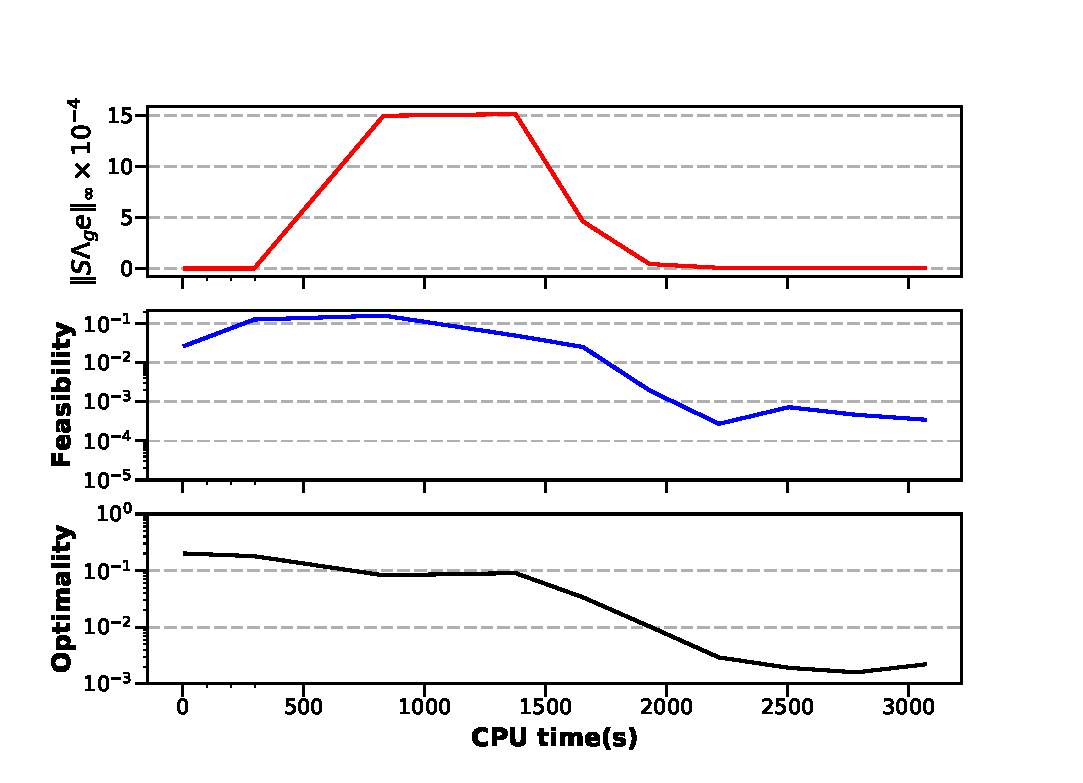
\includegraphics[clip,trim=0 0 0 30, width=1.0\textwidth]{./figs/chap7_aso/kona/L1_192_comp_opt_feas.eps} }  \\
  % \hspace{1em}
  \subfloat[\label{fig:kona192cd}]{
   \includegraphics[clip,trim=0 0 0 30, width=1.0\textwidth]{./figs/chap7_aso/kona/L1_192_cdlm.eps} }
  % \hspace{1em}
   \caption{Convergence histories for L1 grid, no. of design 192 \label{fig:kona_192}}
\end{figure}

\begin{figure}[H]
  \centering
   \subfloat[\label{fig:kona480opt}]{
   \includegraphics[clip,trim=0 0 0 30,width=1.0\textwidth]{./figs/chap7_aso/kona/L1_480_comp_opt_feas.eps} }  \\
  % \hspace{1em}
  \subfloat[\label{fig:kona480cd}]{
   \includegraphics[clip,trim=0 0 0 30,width=1.0\textwidth]{./figs/chap7_aso/kona/L1_480_cdlm.eps} }
  % \hspace{1em}
   \caption{Convergence histories for L1 grid, no. of design 480 \label{fig:kona_480}}
\end{figure}
\begin{figure}[H]
  \centering
   \subfloat[\label{fig:kona768opt}]{
   \includegraphics[clip,trim=0 0 0 30,width=1.0\textwidth]{./figs/chap7_aso/kona/L1_768_comp_opt_feas.eps} } \\
  % \hspace{1em}
  \subfloat[\label{fig:kona768cd}]{
   \includegraphics[clip,trim=0 0 0 30,width=1.0\textwidth]{./figs/chap7_aso/kona/L1_768_cdlm.eps} }
%   \hspace{1em}
   \caption{Convergence histories for L1 grid, no. of design 768 \label{fig:kona_768}}
\end{figure}


\begin{figure}[H]
  \centering
   \subfloat[\label{fig:sn192opt}]{
   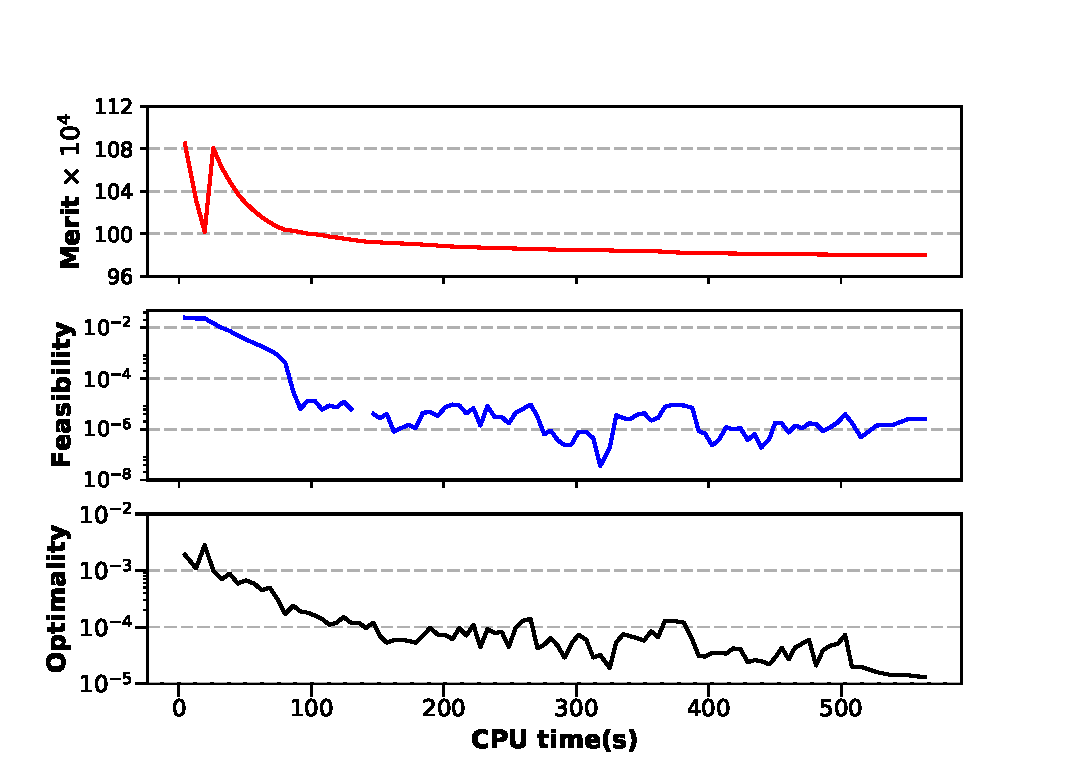
\includegraphics[clip,trim=0 0 0 30,width=1.0\textwidth]{./figs/chap7_aso/snopt/L1_192_opt_feas.eps} }\\
  % \hspace{1em}
  \subfloat[\label{fig:sn192cd}]{
   \includegraphics[clip,trim=0 0 0 30,width=1.0\textwidth]{./figs/chap7_aso/snopt/L1_192_cdlm.eps} }
  % \hspace{1em}
   \caption{Convergence histories for L1 grid, no. of design 192 \label{fig:sn_192}}
\end{figure}

\begin{figure}[H]
  \centering
   \subfloat[\label{fig:sn480opt}]{
   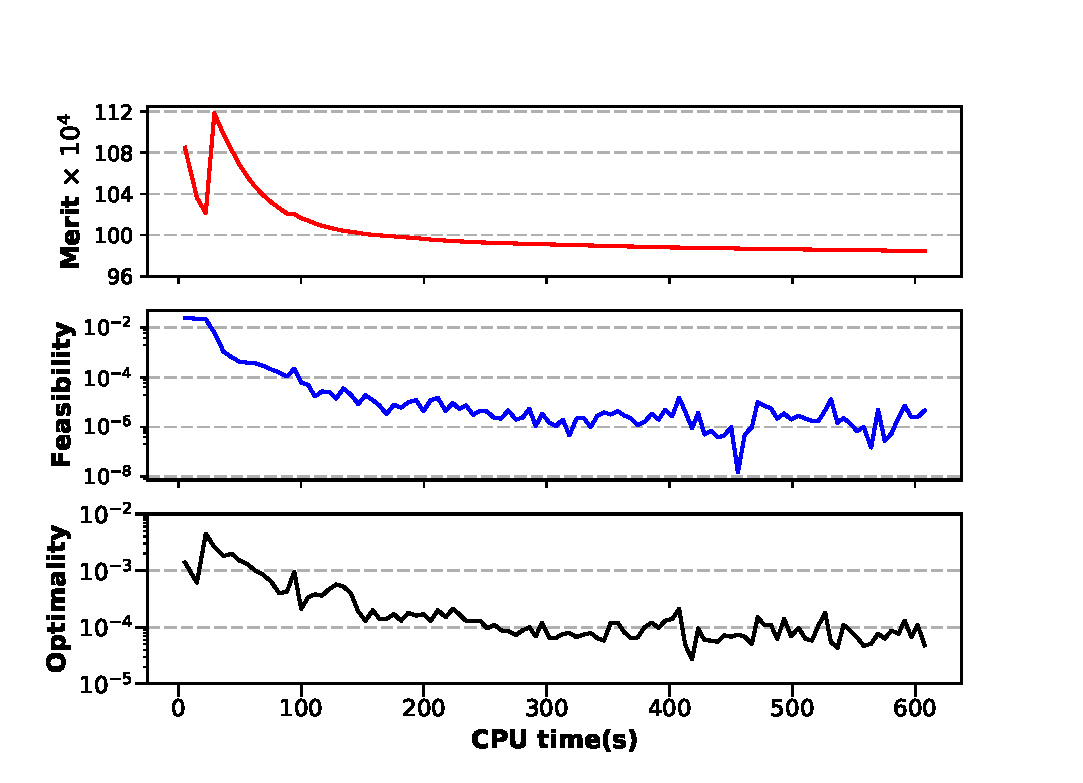
\includegraphics[clip,trim=0 0 0 30,width=1.0\textwidth]{./figs/chap7_aso/snopt/L1_480_opt_feas.eps} }\\
  % \hspace{1em}
  \subfloat[\label{fig:sn480cd}]{
   \includegraphics[clip,trim=0 0 0 30,width=1.0\textwidth]{./figs/chap7_aso/snopt/L1_480_cdlm.eps} }
  % \hspace{1em}
   \caption{Convergence histories for L1 grid, no. of design 480 \label{fig:sn_480}}
\end{figure}
\begin{figure}[H]
  \centering
   \subfloat[\label{fig:sn768opt}]{
   \includegraphics[clip,trim=0 0 0 30,width=1.0\textwidth]{./figs/chap7_aso/snopt/L1_768_opt_feas.eps}}\\
  % \hspace{1em}
  \subfloat[\label{fig:sn768cd}]{
   \includegraphics[clip,trim=0 0 0 30,width=1.0\textwidth]{./figs/chap7_aso/snopt/L1_768_cdlm.eps} }
%   \hspace{1em}
   \caption{Convergence histories for L1 grid, no. of design 768 \label{fig:sn_768}}
\end{figure}

\subsubsection{Discussion}
The results above demonstrate that the homotopy RSNK method can solve 
a difficult, large-scale aerodynamic shape optimization problem.
However, its computational performance is disappointing on this problem relative to SNOPT. 
Kona's poor performance is largely due to the computational expense of forming the SVD-based 
preconditioner. This can be explained by the fact that one Lanczos iteration in the preconditioner involves  
one Jacobian vector product and one vector Jacobian product for both the equality and inequality constraints. This makes the SVD approximation expensive, because it uses 20 Lanczos iterations at each optimization iteration point. In addition, the inequality constraints consist of 750 thickness constraints, 1 volume constraint,  and 2 nonlinear aerodynamic constraints. Thus, the preconditioner is lumping the nonlinear and linear inequality constraints together when computing the Jacobian-vector and vector-Jacobian products, which makes the SVD approximation less effective at approximating the nonlinear part.  Rather than using the SVD to approximate the linear constraints, it would be advantageous to use the explicit linear Jacobians. 

%Because the there are only two nonlinear aerodynamic constraints in this problem, $CL$ and $CMy$, while the rest of the inequality constraints are large amount of linear geometric constraints, $750$ thickness constraints, $1$ volume constraint, the preconditioner is lumping the nonlinear and linear inequality constraints together when making SVD approximations.  The parameters used in Kona are listed in Appendix~\ref{tab:param}.  

%%%%%%%%%%%%%%%%%%%%%%%%%%%%%%%%%%%%

%%% Local Variables: 
%%% mode: latex
%%% TeX-master: t
%%% End: 
